\documentclass{article}
\usepackage{geometry}
\geometry{
	a4paper,
	left=2.5cm,
	right=2.5cm,
	top=2.5cm,
	bottom=2.5cm,
	headheight=13.6pt
}
% 最简单、最稳定的中文方案（自动适配系统，永不报错）
\usepackage[UTF8, scheme=plain]{ctex}
% 设置英文默认字体为 Times New Roman
\usepackage{fontspec}
\setmainfont{Times New Roman}
\usepackage{amsmath}
\usepackage{amssymb}
\usepackage{booktabs}
\usepackage{caption}
\usepackage{setspace}
\doublespacing
\setlength{\parskip}{4pt}
\usepackage{array}
\usepackage{listings}
\usepackage{graphicx}
\usepackage{enumitem}
\usepackage{subcaption}
\usepackage{multirow}
\usepackage{mathrsfs}
\usepackage{bm}
\usepackage{xcolor}
\usepackage{colortbl}
\usepackage{tikz}
\usepackage{tikz-3dplot}
\usetikzlibrary{
	arrows.meta,
	calc,
	patterns,
	decorations.pathmorphing,
	backgrounds,
	positioning,
	fit,
	shapes.geometric,
	intersections,
	through,
	angles,
	quotes,
	plotmarks
}
%目录超链接
\usepackage{hyperref}
\hypersetup{
	colorlinks=true,
	linkcolor=black,
	filecolor=magenta,
	urlcolor=cyan,
}
\usepackage{tocloft}
\setlength{\cftbeforesecskip}{2ex}
\setlength{\cftbeforesubsecskip}{1ex}
\setlength{\cftbeforesubsubsecskip}{1ex}
% 定义代码颜色
\definecolor{codegreen}{rgb}{0,0.6,0}
\definecolor{NavyBlue}{RGB}{0,0,128}
\definecolor{PineGreen}{RGB}{1,121,111}
% 配置 listings 环境
\lstset{
	language=TeX,
	tabsize=4,
	captionpos=b,
	numbers=left,
	numbersep=1em,
	sensitive=true,
	showtabs=false,
	frame=shadowbox,
	breaklines=true,
	keepspaces=true,
	showspaces=false,
	showstringspaces=false,
	breakatwhitespace=false,
	basicstyle=\ttfamily\normalsize,
	keywordstyle=\color{NavyBlue},
	commentstyle=\color{codegreen},
	numberstyle=\color{black},
	stringstyle=\color{PineGreen!90!black},
	rulesepcolor=\color{red!20!green!20!blue!20},
	escapeinside={/@}{@/},
}
% 自定义颜色
\definecolor{LightGreen}{rgb}{0.9, 0.95, 0.9}
\definecolor{LightBlue}{RGB}{229, 238, 255}
\definecolor{LightPink}{RGB}{255, 229, 237}
\definecolor{DarkRed}{RGB}{169,0,0}
\definecolor{DarkGreen}{RGB}{0,110,12}
\definecolor{SkyBlue}{RGB}{0,114,255}
% 自定义环境 无缩进
\newenvironment{knowledge}[1]{%
	\noindent{%
		\normalfont\bfseries\color{DarkRed} #1}\hskip 0.5em%
	\color{DarkRed}%
}{%
	\par\color{black}%
}
\newenvironment{question}[1][]{%
	\noindent
	\ifx\relax#1\relax\else
	{%
		\normalfont\color{DarkGreen} #1}\hskip 0.5em%
	\fi
	\color{DarkGreen}%
}{%
	\ifhmode\fi\color{black}%
}
\newcommand{\category}[1]{%
	\noindent{%
		\normalfont\bfseries\color{SkyBlue} #1}\hskip 0.5em}
\captionsetup[table]{
	justification=centering,
	labelsep=quad,
	font={bf}
}
\captionsetup[figure]{
	justification=centering,
	labelsep=quad,
	font={bf}
}
\captionsetup[subfigure]{
	font={bf}
}
\begin{document}
	
	\begin{center}
		
		{\LARGE \textbf{零基础偏微分方程笔记}} \\[0.5cm]
		{\large {\kaishu 石继楷 \quad 编写}} \\[0.3cm]
		{\normalsize \today}
	\end{center}
	\tableofcontents
	\newpage
	
	\section{第一讲\quad 偏微分方程的基本概念}
	\subsection{PDE 的定义与记号}
	\begin{knowledge}{偏微分方程（PDE）}
		
		包含一个未知函数、两个或更多自变量以及该未知函数偏导数的方程，称为偏微分方程.
		
		记号约定：
		\begin{enumerate}[label=\arabic*$^\circ$, left=0pt]
			
			\item $U$ 为 $\mathbb{R}^n$ 中的开集，$U \subseteq \mathbb{R}^n$.
			\item 未知函数 $u: U \to \mathbb{R}$，$u(x) = u(x_1, x_2, \dots, x_n)$，$x = (x_1,\dots,x_n) \in U$.
			\item 偏导数：$u_{x_i} = \dfrac{\partial u}{\partial x_i}$，$u_{x_i x_j} = \dfrac{\partial^2 u}{\partial x_j \partial x_i}$.
		\end{enumerate}
	\end{knowledge}
	\begin{knowledge}{多重指标记号}
		
		设 $\alpha = (\alpha_1, \dots, \alpha_n)$ 为 $n$ 维非负整数组（称为多重指标），其阶数定义为
		\[
		|\alpha| = \alpha_1 + \dots + \alpha_n.
		\]
		相应的高阶偏导数记为
		\[
		D^\alpha u = \frac{\partial^{|\alpha|} u}{\partial^{\alpha_1} x_1 \, \partial^{\alpha_2} x_2 \cdots \partial^{\alpha_n} x_n} = \frac{\partial^{|\alpha|} u}{\partial x_1^{\alpha_1} \cdots \partial x_n^{\alpha_n}}.
		\]
		并把所有 $k$ 阶偏导数构成的集合记为
		\[
		D^k u = \{ D^\alpha u : |\alpha| = k \}.
		\]
		特别地，一阶偏导数组成的向量称为梯度：
		\[
		Du = (u_{x_1}, \dots, u_{x_n}) = \nabla u.
		\]
	\end{knowledge}
	\subsection{线性偏微分方程}
	\begin{knowledge}{线性与齐次}
		
		形如
		\[
		\sum_{|\alpha| \leq k} a_\alpha(x) D^\alpha u(x) = f(x)
		\]
		的方程称为 $k$ 阶线性偏微分方程，其中 $a_\alpha$，$f$ 为给定函数.
		
		"线性"指未知函数 $u$ 及其各阶偏导数均以一次幂线性出现，方程中不出现 $\|Du\|^2$，$\sin u$ 等非线性项.
		
		若 $f \equiv 0$，称该 PDE 为齐次的；否则称为非齐次的.
	\end{knowledge}
	
	\section{第二讲\quad 传输方程}
	\subsection{齐次方程与特征线法}
	\begin{knowledge}{传输方程}
		
		设 $\vec{b} = (b_1,\dots,b_n) \in \mathbb{R}^n$ 为常向量，传输方程为
		\[
		u_t + \vec{b} \cdot Du = 0, \quad (x,t) \in \mathbb{R}^n \times (0, +\infty).
		\]
		改写为内积形式
		\[
		(1, \vec{b}) \cdot (u_t, Du) = 0,
		\]
		即 $u$ 沿空间-时间方向 $(1, \vec{b})$ 的方向导数为零. 特征线法的思想是：选取适当曲线（特征线），把 PDE 化为沿该曲线的常微分方程.
	\end{knowledge}
	\category{特征线法}
	\begin{question}{沿特征线求导}
		
		取特征线 $x(t) = \vec{b} t + x_0$（即 $x = bt + x_0$），验证 $u$ 沿特征线为常数.
	\end{question}
	
	\begin{minipage}[t]{0.7\textwidth}
		
		沿特征线对 $t$ 求全导数：
		\[
		\frac{d}{dt} u(x(t), t) = \sum_{i=1}^n u_{x_i}(x(t), t) \cdot \frac{d x_i(t)}{dt} + u_t(x(t), t)
		\]
		\[
		= \sum_{i=1}^n b_i u_{x_i}(x(t), t) + u_t(x(t), t) = \vec{b} \cdot Du + u_t = 0.
		\]
		$\therefore u(x(t), t)$ 沿特征线为常数.
		
		$\therefore u(x, t) = u(x_0, 0)$，其中由 $x = \vec{b} t + x_0$ 得 $x_0 = x - \vec{b} t$，即
		\[
		u(x, t) = u(x - \vec{b} t, 0), \quad \forall x \in \mathbb{R}^n,\ t > 0.
		\]
	\end{minipage}
	\hfill
	\begin{minipage}[t]{0.3\textwidth}
		
		\centering
		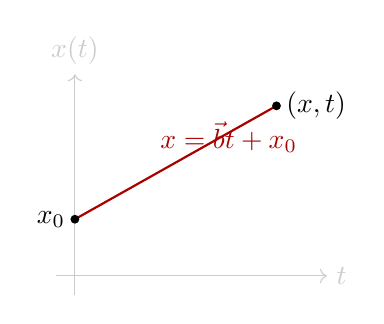
\begin{tikzpicture}[scale=0.8, baseline=(current bounding box.north)]
			\draw[->, gray!40] (-0.3,0) -- (4,0) node[right] {$t$};
			\draw[->, gray!40] (0,-0.3) -- (0,3.2) node[above] {$x(t)$};
			\draw[thick, DarkRed] (0,0.9) -- (3.2,2.7);
			\fill (0,0.9) circle (2pt) node[left] {$x_0$};
			\fill (3.2,2.7) circle (2pt) node[right] {$(x,t)$};
			\node[above right, DarkRed] at (1.2,1.8) {$x=\vec{b}t+x_0$};
		\end{tikzpicture}
	\end{minipage}
	\subsection{初值问题与行波解}
	\begin{knowledge}{初值问题}
		
		考虑初值问题
		\[
		\begin{cases}
			u_t + \vec{b} \cdot Du = 0 & \mathbb{R}^n \times (0,+\infty) \\
			u = g & \mathbb{R}^n \times \{t=0\}
		\end{cases}
		\]
		即 $t=0$ 时 $u(x,0) = g(x)$. 由特征线结论立得
		\[
		u(x,t) = g(x - \vec{b} t).
		\]
		物理意义：初始波形 $g$ 以速度 $\vec{b}$ 整体平移，故称行波解.
	\end{knowledge}
	\begin{question}{验证}
		
		$u(x,t) = g(x-\vec{b}t)$ 确为方程的解.
	\end{question}
	
	由链式法则 $u_t = -\vec{b} \cdot Dg(x-\vec{b}t)$，$Du = Dg(x-\vec{b}t)$，
	\[
	u_t + \vec{b} \cdot Du = -\vec{b} \cdot Dg(x-\vec{b}t) + \vec{b} \cdot Dg(x-\vec{b}t) = 0.
	\]
	\subsection{变系数情形}
	\category{特征线为指数曲线}
	\begin{question}{特殊方程}
		
		\[
		\begin{cases}
			u_t + x \cdot Du = 0 & \mathbb{R}^n \times (0,+\infty) \\
			u = g & \mathbb{R}^n \times \{t=0\}
		\end{cases}
		\]
		此时系数非常向量，特征线满足 $\dfrac{dx(t)}{dt} = x(t)$.
	\end{question}
	
	\begin{minipage}[t]{0.7\textwidth}
		
		解特征方程：
		\[
		\frac{dx(t)}{dt} = x(t) \implies x(t) = x_0 e^t, \quad x_0 = \frac{x}{e^t} = x e^{-t}.
		\]
		沿特征线求导：
		\[
		\frac{d}{dt} u(x(t), t) = \frac{dx(t)}{dt} \cdot Du(x(t), t) + u_t(x(t), t) = x(t) \cdot Du(x(t),t) + u_t(x(t),t) = 0.
		\]
		$\Rightarrow u(x(t), t)$ 为常数.
		\[
		u(x,t) = u(x_0, 0) = g(x_0) = g\left(\frac{x}{e^t}\right) = g(x e^{-t}).
		\]
	\end{minipage}
	\hfill
	\begin{minipage}[t]{0.3\textwidth}
		
		\centering
		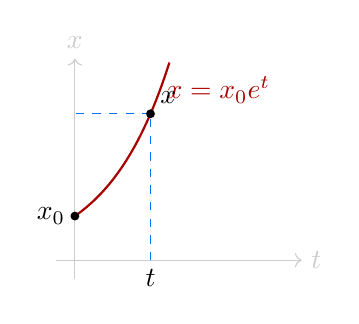
\begin{tikzpicture}[scale=0.8, baseline=(current bounding box.north)]
			\draw[->, gray!40] (-0.3,0) -- (3.6,0) node[right] {$t$};
			\draw[->, gray!40] (0,-0.3) -- (0,3.2) node[above] {$x$};
			\draw[thick, DarkRed, domain=0:1.5, smooth, samples=60, variable=\t] plot ({\t}, {0.7*exp(\t)});
			\fill (0,0.7) circle (2pt) node[left] {$x_0$};
			\node[right, DarkRed] at (1.3,2.7) {$x=x_0e^t$};
			\draw[dashed, SkyBlue] (1.2,0) -- (1.2,{0.7*exp(1.2)});
			\draw[dashed, SkyBlue] (1.2,{0.7*exp(1.2)}) -- (0,{0.7*exp(1.2)});
			\fill (1.2,{0.7*exp(1.2)}) circle (2pt) node[above right] {$x$};
			\node[below] at (1.2,0) {$t$};
		\end{tikzpicture}
	\end{minipage}
	\subsection{非齐次问题}
	\begin{knowledge}{非齐次传输方程}
		
		\[
		\begin{cases}
			u_t + \vec{b} \cdot Du = f & \mathbb{R}^n \times (0,+\infty) \\
			u = g & \mathbb{R}^n \times \{t=0\}
		\end{cases}
		\]
		源项 $f$ 表示外部输入. 仍沿特征线 $x(s) = \vec{b} s + x_0$ 求解.
	\end{knowledge}
	\begin{minipage}[t]{0.7\textwidth}
		
		沿特征线（以 $s$ 为参数）：
		\[
		\frac{d}{ds} u(x(s), s) = \vec{b} \cdot Du(x(s), s) + u_t(x(s), s) = f(x(s), s).
		\]
		两边对 $s$ 从 $0$ 到 $t$ 积分：
		\[
		u(x(t), t) - u(x_0, 0) = \int_0^t f(x(s), s)\, ds.
		\]
		由 $x = \vec{b} t + x_0$ 得 $x_0 = x - \vec{b} t$，$x(s) = \vec{b} s + x - \vec{b} t$，故
		\[
		u(x, t) = g(x - \vec{b} t) + \int_0^t f(\vec{b} s + x - \vec{b} t, s)\, ds.
		\]
		即解等于齐次行波解加上源项沿特征线的累积（Duhamel 原理）.
	\end{minipage}
	\hfill
	\begin{minipage}[t]{0.3\textwidth}
		
		\centering
		\begin{tikzpicture}[scale=0.8, baseline=(current bounding box.north)]
			\draw[->, gray!40] (-0.3,0) -- (4,0) node[right] {$t$};
			\draw[->, gray!40] (0,-0.3) -- (0,3.2) node[above] {$x$};
			\draw[thick, DarkRed] (0.4,0.6) -- (3.4,2.6);
			\fill (0.4,0.6) circle (2pt) node[below left] {$(x_0,0)$};
			\fill (3.4,2.6) circle (2pt) node[right] {$(x,t)$};
			\fill (1.9,1.6) circle (2pt) node[below right] {$(x(s),s)$};
			\node[above left, DarkRed] at (1.7,1.7) {特征线};
			\draw[dashed, SkyBlue] (3.4,2.6) -- (3.4,0);
			\node[below] at (3.4,0) {$t$};
		\end{tikzpicture}
	\end{minipage}
	
	\section{第三讲\quad Laplace 方程与 Poisson 方程}
	\subsection{方程与调和函数}
	\begin{knowledge}{Laplace 方程与 Poisson 方程}
		
		Laplace 方程：
		\[
		\Delta u = 0, \quad u = u(x_1, \dots, x_n),
		\]
		其中 $\Delta u = \sum_{i=1}^n u_{x_i x_i}$ 为 Laplace 算子.
		
		Poisson 方程（非齐次）：
		\[
		-\Delta u = f.
		\]
	\end{knowledge}
	\begin{knowledge}{调和函数}
		
		开集 $U$ 上满足 $\Delta u = 0$ 的 $C^2$ 函数 $u$ 称为调和函数.
	\end{knowledge}
	\subsection{物理背景与 Gauss-Green 公式}
	\begin{minipage}[t]{0.7\textwidth}
		
		\begin{knowledge}{物理意义}
			
			设 $u$ 表示某化学物质在 $x$ 处的浓度，$F$ 表示通量密度（向量值函数）. 由 Fick 定律：
			\[
			F = -c \cdot Du \quad (c > 0 \text{ 为扩散系数}).
			\]
			平衡状态时，任取闭包含于 $U$ 的区域 $V \subseteq U$，通过边界 $\partial V$ 的净流量为零（$\nu$ 为单位外法向）：
			\[
			\int_{\partial V} F \cdot \nu \, dS = 0.
			\]
		\end{knowledge}
		\begin{knowledge}{Gauss-Green 公式}
			
			设 $V$ 为具有光滑边界的有界区域，$u \in C^1(\bar{V})$，则
			\[
			\int_V u_{x_i} \, dx = \int_{\partial V} u \, \nu^i \, dS, \quad i = 1, \dots, n,
			\]
			其中 $\nu = (\nu^1, \dots, \nu^n)$ 为 $\partial V$ 的单位外法向.
		\end{knowledge}
	\end{minipage}
	\hfill
	\begin{minipage}[t]{0.3\textwidth}
		
		\centering
		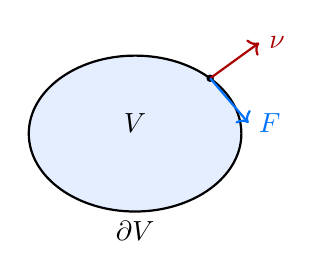
\begin{tikzpicture}[scale=0.9, baseline=(current bounding box.north)]
			\draw[thick, fill=LightBlue] (0,0) ellipse (1.5 and 1.1);
			\node at (0,0.15) {$V$};
			\node[below] at (0,-1.1) {$\partial V$};
			\coordinate (P) at (1.06,0.78);
			\fill (P) circle (1.5pt);
			\draw[->, thick, DarkRed] (P) -- (1.75,1.28) node[right] {$\nu$};
			\draw[->, thick, SkyBlue] (P) -- (1.6,0.15) node[right] {$F$};
		\end{tikzpicture}
	\end{minipage}
	\begin{question}{由平衡律导出 Laplace 方程}
		
		将 Gauss-Green 公式逐分量应用于向量场 $F$（即散度定理）：
		\[
		\int_{\partial V} F \cdot \nu \, dS = \sum_{i=1}^n \int_{\partial V} F_i \, \nu^i \, dS = \sum_{i=1}^n \int_V \frac{\partial F_i}{\partial x_i} \, dx = \int_V \operatorname{div} F \, dx.
		\]
		代入 $F = -c \, Du$：
		\[
		\int_{\partial V} F \cdot \nu \, dS = \sum_{i=1}^n \int_V -c \, u_{x_i x_i} \, dx = -c \int_V \Delta u \, dx.
		\]
		由平衡律，上式对任意 $V$ 均为 $0$；又 $\Delta u$ 连续，
		\[
		\therefore \Delta u = 0.
		\]
		即平衡态浓度必为调和函数.
	\end{question}
	\subsection{基本解：球对称约化}
	\begin{minipage}[t]{0.7\textwidth}
		
		\begin{knowledge}{球对称约化}
			
			希望找到对称性好的解：只依赖于长度 $r = |x| = \sqrt{x_1^2 + \dots + x_n^2}$. 设
			\[
			u(x) = v(r), \quad v: \mathbb{R} \to \mathbb{R}, \ v \text{ 待定}.
			\]
		\end{knowledge}
		\begin{question}{计算 $\Delta u$}
			
			基本关系：
			\[
			\frac{\partial r}{\partial x_i} = \frac{1}{2}(x_1^2 + \dots + x_n^2)^{-\frac{1}{2}} \cdot 2x_i = \frac{x_i}{r}.
			\]
			$\therefore u_{x_i} = v'(r) \cdot \dfrac{x_i}{r}$.
			\[
			u_{x_i x_i} = v''(r) \cdot \frac{x_i^2}{r^2} + v'(r)\left(\frac{1}{r} - \frac{x_i^2}{r^3}\right).
			\]
			求和（注意 $\sum_{i=1}^n x_i^2 = r^2$）：
			\[
			\Delta u = \sum_{i=1}^n u_{x_i x_i} = v''(r) + v'(r)\left(\frac{n}{r} - \frac{1}{r}\right) = v''(r) + \frac{n-1}{r} v'(r) = 0.
			\]
		\end{question}
	\end{minipage}
	\hfill
	\begin{minipage}[t]{0.3\textwidth}
		
		\centering
		\begin{tikzpicture}[scale=0.8, baseline=(current bounding box.north)]
			\draw[->, gray!40] (-2.2,0) -- (2.4,0) node[right] {$x_1$};
			\draw[->, gray!40] (0,-2.2) -- (0,2.4) node[above] {$x_2$};
			\draw[thick, DarkRed] (0,0) circle (1.6);
			\draw[dashed, gray] (0,0) circle (0.9);
			\draw[->, thick, SkyBlue] (0,0) -- (1.13,1.13);
			\fill (1.13,1.13) circle (2pt) node[above right] {$x$};
			\fill (0,0) circle (1.5pt) node[below left] {$O$};
			\node[SkyBlue] at (0.8,0.35) {$r=|x|$};
			\node[DarkRed, below] at (0,-1.9) {等值线（$n=2$ 示意）};
		\end{tikzpicture}
	\end{minipage}
	\begin{knowledge}{求解 ODE}
		
		\[
		\therefore \frac{v''(r)}{v'(r)} = \frac{1-n}{r}.
		\]
		\[
		\therefore (\log v'(r))' = \frac{1-n}{r}.
		\]
		积分：
		\[
		\log v'(r) = (1-n)\log r + C_1, \quad v'(r) = C_2 \cdot r^{1-n}.
		\]
		再积分：
		\begin{enumerate}[label=\arabic*$^\circ$, left=0pt]
			
			\item $n=2$：$v(r) = C_2 \cdot \ln r + C_3$.
			\item $n \geq 3$：$v(r) = C_2 \cdot \dfrac{1}{r^{n-2}} + C_3$.
		\end{enumerate}
	\end{knowledge}
	\begin{knowledge}{基本解}
		
		取适当常数，定义基本解：
		\[
		\Phi(x) =
		\begin{cases}
			-\dfrac{1}{2\pi} \ln|x|, & n=2, \\[8pt]
			\dfrac{1}{n(n-2)\alpha(n)} \cdot \dfrac{1}{|x|^{n-2}}, & n \geq 3,
		\end{cases}
		\]
		其中 $\alpha(n)$ 为 $\mathbb{R}^n$ 中单位球体积：
		\[
		\alpha(n) = \int_{|x|<1} dx = \frac{\pi^{\frac{n}{2}}}{\Gamma\left(\frac{n}{2}+1\right)}.
		\]
		注：$\Phi$ 在 $\mathbb{R}^n \setminus \{0\}$ 上调和，且在分布意义下满足 $-\Delta \Phi = \delta_0$，即原点处单位点源的响应.
	\end{knowledge}
	\subsection{Poisson 方程的解}
	\begin{knowledge}{定理（Poisson 方程的解）}
		
		设 $f \in C_c^2(\mathbb{R}^n)$，即 $f$ 二次连续可微且具有紧支集（$\{f \neq 0\}$ 的闭包为紧集）. 定义
		\[
		u(x) = \int_{\mathbb{R}^n} \Phi(x-y) f(y)\, dy, \quad x \in \mathbb{R}^n.
		\]
		则 $u$ 是 Poisson 方程的解，即满足：
		\begin{enumerate}[label=\arabic*$^\circ$, left=0pt]
			
			\item $u \in C^2(\mathbb{R}^n)$；
			\item $-\Delta u = f$ 在 $\mathbb{R}^n$ 上成立.
		\end{enumerate}
		注：该积分即卷积 $u = \Phi * f$；证明需验证积分与二阶导数可交换，此处从略.
	\end{knowledge}
	
\end{document}